\section{Udstyr og testlokation}
\label{UdstyrLokationSocialAccept}
%
Da det kræver tre forskellige lokationer for at afvikle testen vil listen af det nødvendige udstyr præsenteres i forhold til lokation. De tre lokationer er; B5-106 Målerum Q hvor værten både familiariseres og hvor værten og gæsten samles, foran Målerum Q hvor gæsten instrueres og påbegynder ferieplanlægning og B5-105 Kontrolrum Q hvor testleder 2 styrer musik, præsenterer hints og reagerer på værtens gestikker. Når testleder 1 ikke er sammen med værten, så er testlederen ligeledes i Kontrolrum Q. \blankline
%
På lokation: B5-106 Målerum Q indgår følgende udstyr: 
\begin{itemize}
\item Videokamera + stativ
\item Video med gestikker
\item Bærbar computer til at afspille video
\item Udprintet \textit{cheat sheet} med gestikker
\item Sofa og sofabord
\item Mobiltelefon
\item To højtalere 
\item Musikanlæg
\item Analogt kommunikationskamera\blankline
\noindent
\end{itemize}
%
Videokamera og stativ indgår for dels at optage testpersonen under familiariseringen og dels for at optage begge testpersoner, når de er samlet. Det vælges at optage med et GoPro Hero4 Silver, da det dækker et stort område, det kan optage både billede og lyd og det er forholdvist diskret i forhold til andre videokameraer. GoPro Hero4 Silver placeres på et stativ for at få en optimal vinkel særligt på værten, som skal lave gestikker. Det tilstræbes at vinklen er 45$^{\circ}$ . Video med gestikker præsenteres under familiariseringen af værten, for at gøre værten bekendt med de forskellige gestikker samt hvilken funktion de er tilknyttet. Den bærbare computer bruges af testleder 1 til at afspille videoen med gestikkerne og når testlederen forlader lokalet tages computeren med. Det udprintet \textit{cheat sheet} med gestikker lægges på pladen under sofabordet, så det ikke ligger frit fremme og forefindes i \autoref{app:CheatSheetTilVaerten}. \textit{Cheat sheetet} indgår for at give værten mulighed for at gense gestikkerne i tilfælde af, at testpersonen har glemt dem når gæsten er på besøg og uden at testlederne behøver, at gå ind i lokalet. Sofa og sofabord indgår for at gøre testsituationen mere virkelighedsnær i form af en dagligstue. Det er også her både vært og gæst sidder når ferierne skal planlægges. Mobiltelefonen indgår da denne fungerer som et hint til værten. Det er ikke vigtigt hvilken type mobiltelefon der indgår, men det er vigtigt at alle former for notifikationer slåes fra, så der ikke opstår forvirring. I testen er mobiltelefonen en iPhone 6. De to højtalere indgår fordi der skal afspilles musik både under familiariseringen og når gæsten er på besøg. Det vælges, at de to højtalere skal være BeoLab 6000 fra Bang $\&$ Olufsen. Da der ikke er udarbejdet en prototype af det endelige produkt fra Bang $\&$ Olufsen vælges det, at anvende et musikanlæg fra samme mærke; BeoSound 3200. Under hele testen er anlægget tændt men passivt og der vil ikke afspilles musik derfra, men værten bliver opfordret til at rette sine gestikker mod anlægget, da det potentielt kan blive nødvendigt for at interagere med Bang $\&$ Olufsen's fremtidig musikanlæg. Kommunikationskameraet indgår fordi det skal være muligt for testlederne, at følge med i hvad der foregår inde i lokalet uden at de er der. Det vælges, at kommunikationskameraet skal være analogt for, at sikre at der ikke er en forsinkelse på signalet, både når testleder 1 præsenterer de forskellige hints og når værten reagerer på de forskellige hints ved at gestikulere. Det analoge kommunikationskamera er ophængt på væggen og filmer i fugleperspektiv. \autoref{fig:Testopstilling2} gengiver testopstillingen når både vært og gæst er tilstede. 
%
\begin{figure}[H]
	\centering
	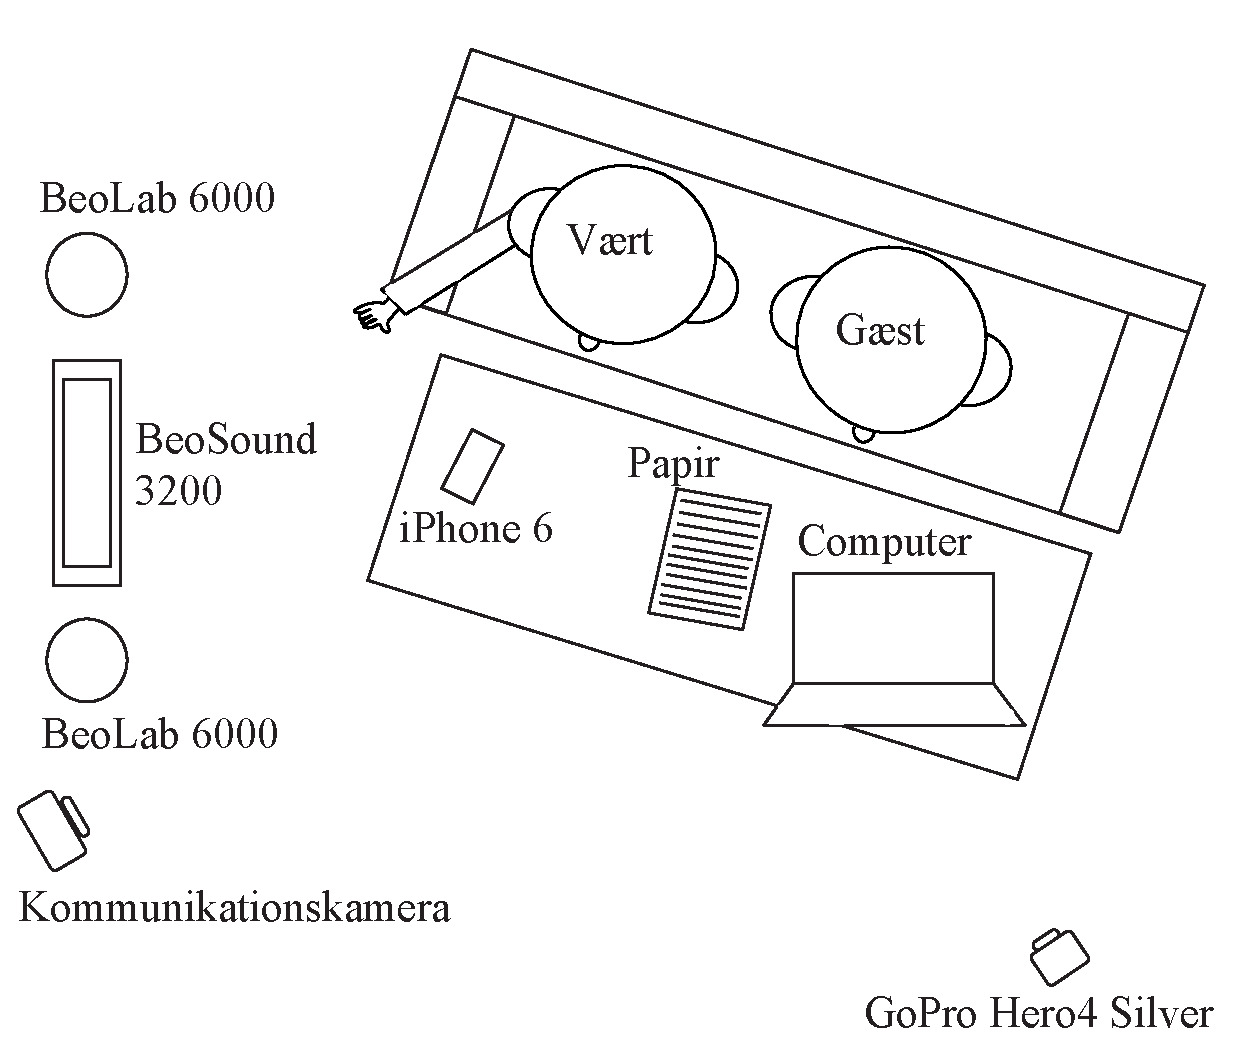
\includegraphics[resolution=300,width=0.8\textwidth]{Test2/Testopstilling2}
	\caption{Testopstilling i Målerum Q hvor placeringen af udstyr samt testpersonernes position fremgår.}
	\label{fig:Testopstilling2}
\end{figure}
\noindent
% 
Som tidligere nævnt skal værten sidde med højre side mod musikanlægget og det analoge kommunikationskamera, da det giver testleder 2 det mest optimale udsyn til gestikkerne. Hvis værten er venstre håndet kan gestikkerne potentielt maskeres af værtens egen krop, hvilket potentielt kan resultere i at testleder 2 ikke kan se gestikkerne og dermed heller ikke kan reagere på gestikkerne. I tilfælde af at værten og gæsten havde byttet plads så ville værten være nødsaget til at række ind foran gæsten for at lave gestikkerne, hvilket antages at være forstyrrende for samtalen mellem vært og gæst, da bevægelsen formentlig vil tiltrække gæstens opmærksomhed. 

Foruden det udstyr, som er listet, så sættes der forplejning frem i form af cookies og Capri-Sonne (juice). Dette gøres for at tilstræbe en hyggelig stemning. \blankline  
%
På lokation: Foran Målerum Q indgår følgende udstyr: 
\begin{itemize}
  \item Bærbar computer med internetforbindelse 
  \item Papir og kuglepen 
  \item Udprintet opsummering af gæstens opgave
  \item Sofa og sofabord\blankline
\noindent
\end{itemize}
%
Den bærbare computer med internetforbindelse indgår for at gæsten kan planlægge de tre forskellige ferier ved at søge på forskellige hjemmesider såsom; trivago.dk, momondo.dk, hotels.com, tripadviser.dk og airbnb.dk, som på forhånd er åbnet. Papir og kuglepen udleveres til gæsten så de har mulighed for at notere ideér til ferierne. Gæsten tager både den bærbare computer og papir samt kuglepen med ind til værten, når de samles. Den udprintet opsummering af gæstens opgave udleveres af testleder 2 for at testpersonen ikke glemmer opgaven og husker hvilke elementer af ferien, der skal planlægges. Opsummeringen af gæstens opgaver forefindes i \autoref{app:OpgaverTilGaesten}. Sofa og sofabord benyttes af både testperson og testleder 2. På \autoref{fig:Testopstilling2Gaest} illustreres testopstillingen ude foran Målerum Q, hvor gæsten bliver introduceret til ferieplanlægning af testleder 2.  
%
\begin{figure}[H]
	\centering
	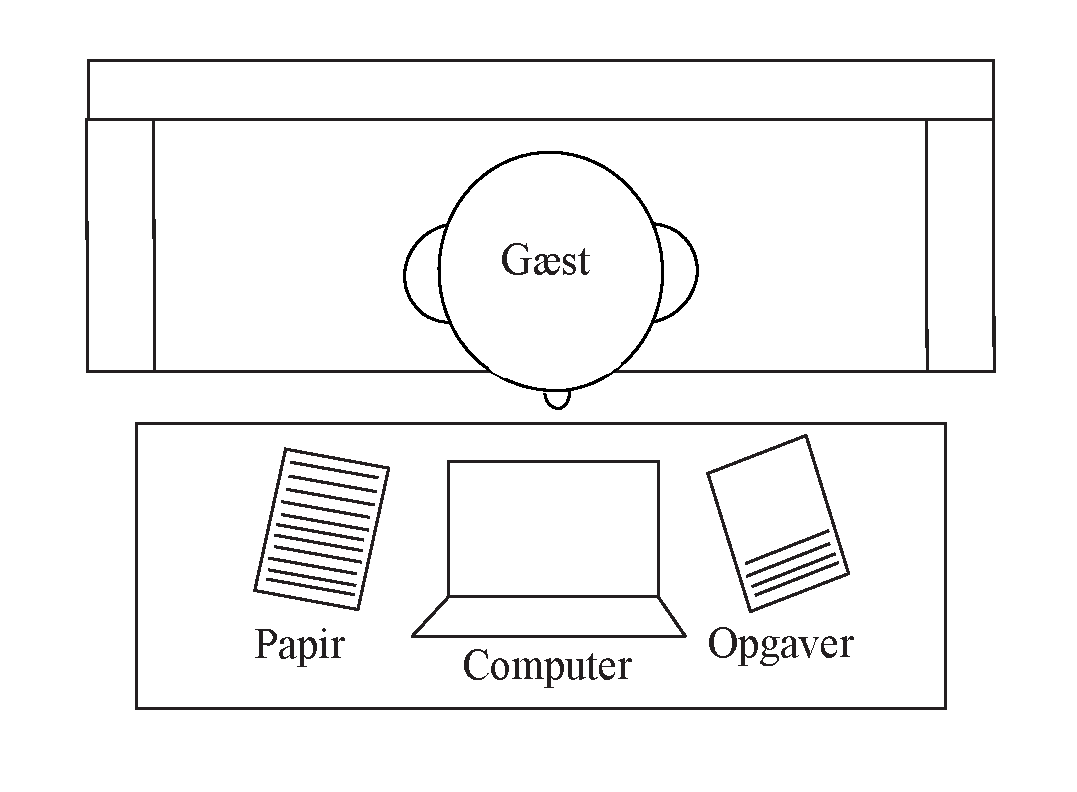
\includegraphics[resolution=300,width=0.8\textwidth]{Test2/Testopstilling2Gaest}
	\caption{Testopstilling foran Målerum Q hvor placeringen af udstyr samt testpersonens position fremgår.}
	\label{fig:Testopstilling2Gaest}
\end{figure}
\noindent
% 
På lokation: B5-105 Kontrolrum Q indgår følgende udstyr:
\begin{itemize}
  \item Bærbar computer med iTunes 12.6
  \item Afspilningsliste til familiarisering uden hints 
  \item Afspilningsliste til familiarisering med hints
  \item Afspilningsliste til testen
  \item \textit{Cheat sheet} over præsentationsrækkefølgen for hints 
  \item Telefon
  \item Forstærker 
  \item Forbindelse til det analoge videokamera
  \item CRT-skærm \blankline
\noindent
\end{itemize}
%
I kontrolrummet indgår den bærbare computer med iTunes 12.6 for, at afspille de tre afspilningslister. Computeren er forbundet til forstærkeren hvorfra volumen blandt andet kan justeres. Forstærkeren er af typen Pioneer Stereo Amplifier A-656. Derudover er forstærkeren koblet til to input kanaler, hvis output afspilles igennem de to BeoLab 6000 højtalere, illustreret på \autoref{fig:Testopstilling2}. \textit{Cheat sheet} over præsentationsrækkefølgen for hints anvendes af testleder 2 for at sikre at testpersonerne, som agerer vært, alle får de samme hints. I kontrolrummet er der ikke krav til hvilken telefon, der skal bruges da det eneste den skal kunne er at ringe til mobiltelefonen inde hos værten. I testen er telefonen en iPhone 5. Da der anvendes et analogt kommunikationskamera til at filme testpersonerne inde i Målerum Q, er det nødvendigt at Kontrolrum Q er i stand til at modtage signalet. Signalet afspilles på CRT-skærmen inde i kontrolrummet, som både gengiver billede og lyd fra det analoge kommunikationskamera. Fjernsynet er et Panasonic Colour TV TX-14B4TC. På \autoref{fig:Testopstilling2Observation} illustreres testopstillingen i Kontrolrum Q hvor begge testledere er til stede.   
%
\begin{figure}[H]
	\centering
	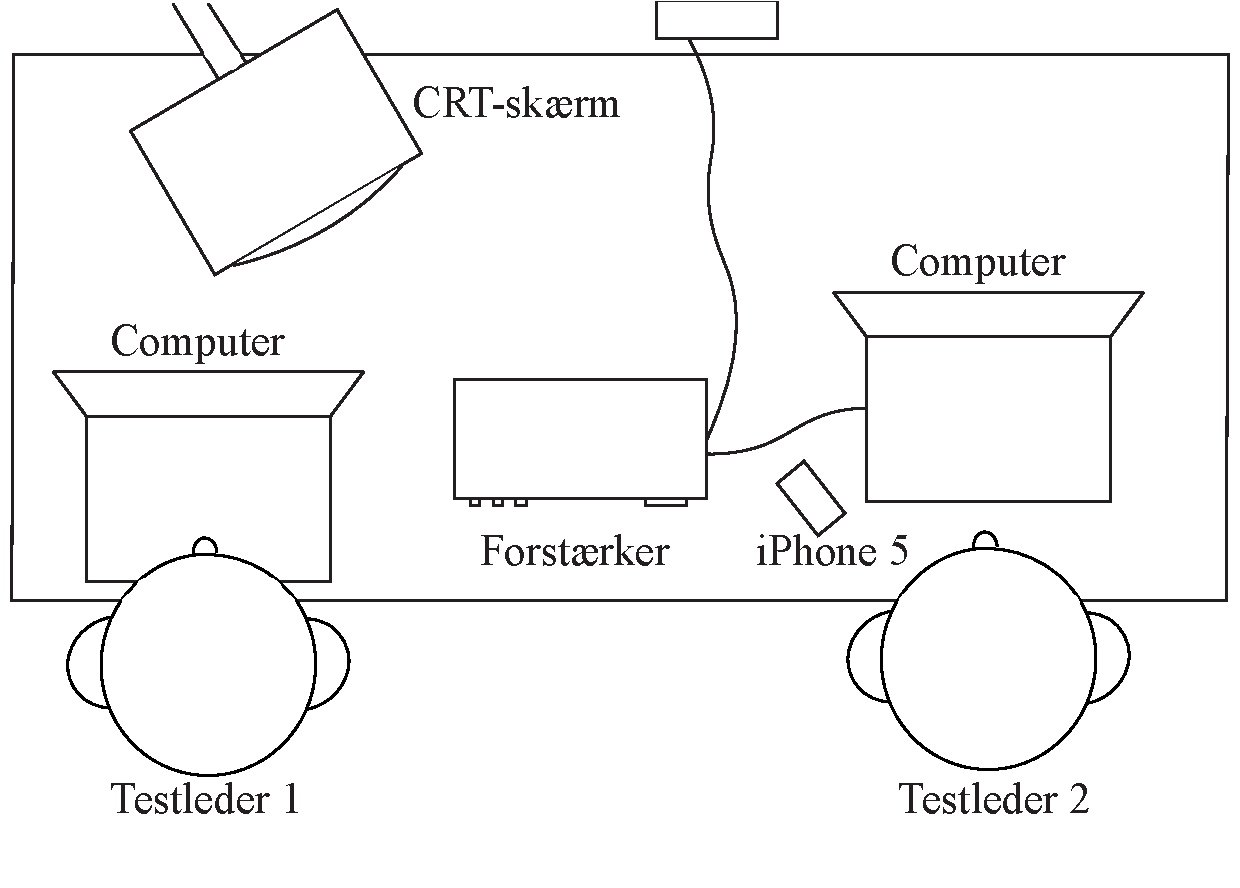
\includegraphics[resolution=300,width=0.8\textwidth]{Test2/Testopstilling2Observation}
	\caption{Testopstilling hvor placeringen af udstyr samt testpersonernes position fremgår.}
	\label{fig:Testopstilling2Observation}
\end{figure}
\noindent
% 


